\section{Numerical Experiments}

We now provide numerical evidence of the efficiency of our method. All the  experiments have been carried out  with Tensorflow 2.7  on a 2021 Macbook pro with 64GB unified memory and Apple M1 Max chip. The code is implemented in Python and run on CPU (10-core) only.  
Throughout the examples, we use the same neural network architecture and training parameters,  given  below:
\begin{enumerate}
\item The feedforward neural network consists of $2$ hidden layers, each having $20 + \text{dim}(\calE)$  nodes  with leaky rectified linear unit (Leaky ReLU) activation function. The output layer uses the standard rectified linear unit (ReLU)  activation. The  bias in the output layer can be used to set  an initial threshold level $\theta_0 \in \R_+$.     In other words, the  threshold function reads
$$G(t,\xi; \theta) = \left(\theta_0 + \theta_1^{\top} G_{-1}(t,\xi; \theta_{-1})\right)^+, \quad (\theta_{-1}, \theta_{0}, \theta_1) = \theta, $$ %, \quad \theta_1 \in \R^{50+\bar{d}}
where  $G_{-1}(t,\xi; \theta_{-1}) \in \R^{20+\bar{d}}$ is the value of the neural network before entering the output layer. From our observations, the algorithm is not sensitive to the initial bias, as long as it is set to a reasonable value.  For example, if the payoff is of the form   $\eqref{eq:payoff}$, we  choose $\theta_0=\frac{3K}{2}$,  $\theta_0=\frac{K}{2}$ for  calls 
and puts
,  respectively. 

\item The number of training iterations is set to $M=3,000$ and batch size to $B = 512$. 
    \item The learning rates $(\zeta_m)$ are obtained from the widely accepted Adam optimizer \cite{Kingma}.
    
    \item  
    If the payoff function is of the form
    $\eqref{eq:payoff}$ (which is the case in all the examples below), the fuzzy boundary width is chosen to be    
    $\epsilon_n = K \sqrt{\V^{\Q}[ \alpha(X^{t_{n-1},1}_{t_n})]}$, $t_n \in \calT_N$. 

     The strike $K$ takes account the scale of the payoff$-$and in turn, the threshold function$-$while  the second in $\epsilon_n$ reflects the typical variation 
     of the  process $\alpha(X)$ between exercise dates.  
\end{enumerate}
The initial price is computed using the sharp boundary and $J= 2^{22} = 4,194,304$ Monte Carlo simulations. 

\subsection{Put Option in the Black-Scholes Model} \label{sec:putBS}
Consider an ATM Bermudan put option ($\varphi(s) = (K-s)^+$) in the Black Scholes model. We take the same parameters as in  Section 4.3.1.2 of \cite{Becker2}, namely
$S_0=K=40$, $r = 6\%$, $\delta = 0\%$, $\sigma = 40\%$, with maturity $T=1$ and  $N=50$ exercise dates.  
As the stock price must reach low values to cross the boundary, we can use importance sampling to make the drift of $S-$which is positive under $\Q-$negative under an equivalent measure. We can for instance set $\lambda \equiv \frac{r-\delta + 0.05}{\sigma}  = 0.275$ so $S$ becomes a submartingale under $\Q^{\lambda}$ with $5\%$ negative drift. Notice that the fuzzy boundary width is approximately equal to $\epsilon = K\sigma \sqrt{T/N}$.  \cref{tab:resultPutBS} summarizes the result, in comparison with the value found by \citet{Becker1}. 

\begin{table}[ht]
  \centering
  \caption{Bermudan Put Option ($N=50$), Black-Scholes model.  
 }
  \begin{tabular}{|c| c| c| c| c|}
 \hline
     Price&  Std& Runtime  & Price in \cite{Becker2}\\
  \hline 
  5.308 & 0.003 &  57.5 & 5.311 \\
  \hline
\end{tabular}
\vspace{2mm}

\scriptsize{
\textit{Notes: The first and second column show the average and standard deviation of ten experiments, respectively. The third column is the average runtime (in seconds) per experiment for the training phase. }}
\label{tab:resultPutBS}
  \end{table}

Figure \ref{fig:putBS} displays the initial boundary (left chart) with the trained one (right chart) compared with the optimal boundary. The latter is obtained using a finite-difference scheme.  

\begin{figure}
    \centering
    \caption{Exercise boundary (Bermudan put,  Black-Scholes model).}
    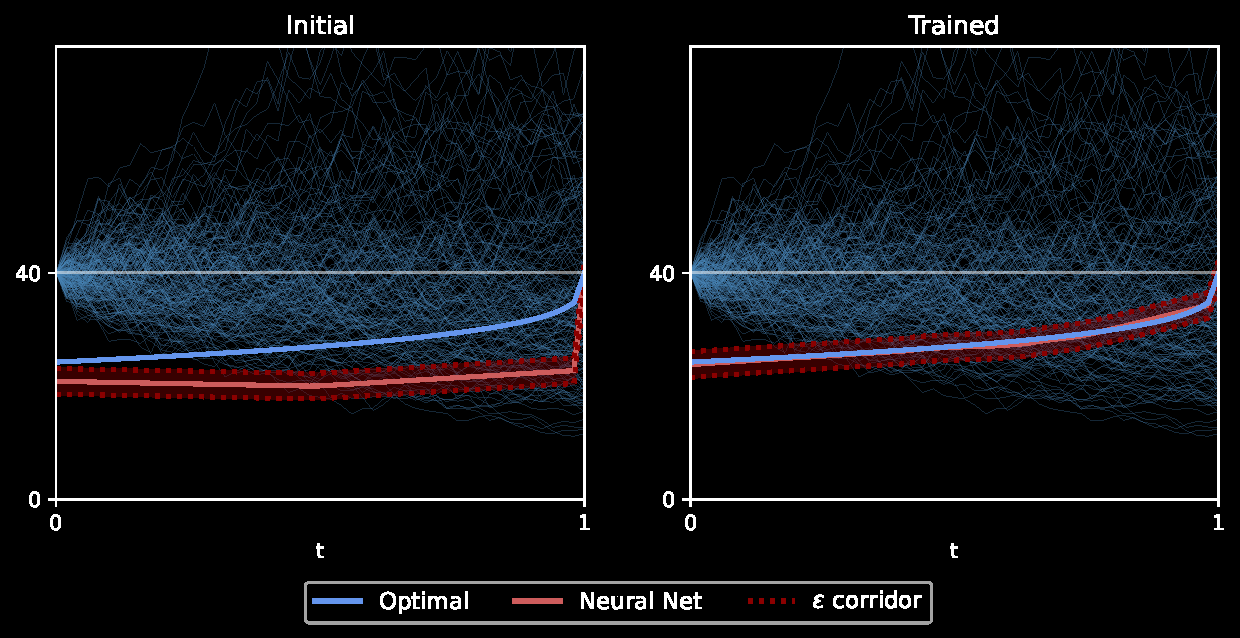
\includegraphics[scale=0.5]{Figures/Bdry 2, lbda=0.275, mu=0.050, N=50.pdf}
    
    \label{fig:putBS}
\end{figure}

\subsection{Put Option in the Heston Model}\label{sec:putHeston}

Consider the Bermudan put option from the previous section ($S_0 =K=40$, $T=1$, $N=50$) in the Heston model. Our goal is to see how stochastic volatility impacts the exercise boundary and  corresponding  price.   
 Let $m=1, \ k=0$ and assume the stock and factor dynamics
\begin{align*}
   \frac{dS_t}{S_t} &= (r-\delta)dt + \sqrt{\calV_t}\  dW_t, \\
   d\calV_t &= (\kappa(\bar{\nu}-\calV_t) - \gamma^{\Q}\calV_t)dt + \sigma_{\calV} \sqrt{\calV_t}\  d\tilde{W}_t, 
\end{align*}
with $\calV_0 = \nu_0 \in \R^2_+$ and $\frac{d\langle W, \tilde{W} \rangle_t}{dt} = \rho  \in  (-1,1)$. 
 
We choose the parameters
 $r = 6\%$, $\delta = 0\%$, $\kappa = 1$, $\nu_0 = \bar{\nu} = (40\%)^2$, $\gamma^{\Q} =0$, $\sigma_{\calV} =10\%$, and $\rho =-0.5$. In particular, 
the Feller condition $\kappa \,  \bar{\nu} \ge  \frac{\sigma_{\calV}^2}{2}$ is satisfied.  

For a fair comparison,  we set the initial value and long term mean of $\calV$ equal to the Black-Scholes variance $\sigma^2$ from \cref{sec:putBS}.   Moreover, we use importance sampling with same Girsanov parameter, i.e. $\lambda \equiv \frac{r-\delta + 0.05}{\sigma}  = 0.275$.

As seen in \cref{ex:vanilla}, the threshold function 
depends on time $t$ and the spot variance $\calV_t =\nu$.  
When $\varphi$ is convex and bounded (which is the case here)   \citet{LambertonHeston} showed that the value function $v(t,x)$, $x=(s,\nu)$, is  non-decreasing in $\nu$ for all $t\in [0,T]$. Consequently, the map $\nu \mapsto f(t,\nu)$ is non-increasing. In figure..., it turns out that the same holds for the trained neural network $G(\cdot,\cdot;\theta^M)$. 
Moreover, as $s \to v(t,s,\nu)$ is non-increasing for fixed $(t,\nu)$,  we expect that the  rectangle $[0,s]\times [0,\nu]$ 
is contained in $\calS_t$ whenever $(s,\nu) \in \calS_t$. This is confirmed in  \cref{fig:heston1}. 

Table \cref{tab:resultPutHeston} compares the price of the claim when the stopping decision exploit the spot variance and when it does not. We observe that the price obtained with the "blind" strategy is significantly lower. Interestingly, the neural network coincides with the optimal boundary in the Black-Scholes model.%, as shown in Figure \cref{fig:heston1}

Figure \cref{fig:heston2} displays a trajectory for $(X,\calV)$ together with the threshold process $G(\cdot,\calV;\theta^M)$. As can be seen, the threshold is typically above the Black-Scholes boundary when $\calV_t$ is below its mean ($0.16$) and vice versa. 

\begin{table}[ht]
  \centering
  \caption{Price of a Bermudan Put Option in the Heston model. \bb{(std to be reduced)}  
 }
  \begin{tabular}{|c| c| c| c| }
 \hline
  Threshold function &  Price&  Std& Runtime  \\
  \hline 
    $f(t,\nu)$ & 5.295 & 0.005 &  57.5 \\
  $f(t)$ & 5.281 & 0.006 &  57.5  \\
  \hline
\end{tabular}
\vspace{2mm}

\scriptsize{
\textit{Notes: The second and third column show the average and standard deviation of ten experiments, respectively.  }}
\label{tab:resultPutHeston}
  \end{table}
  
\begin{figure}[t]
    \centering
     \caption{Stopping and continuation regions (Bermudan put, Heston model).}
    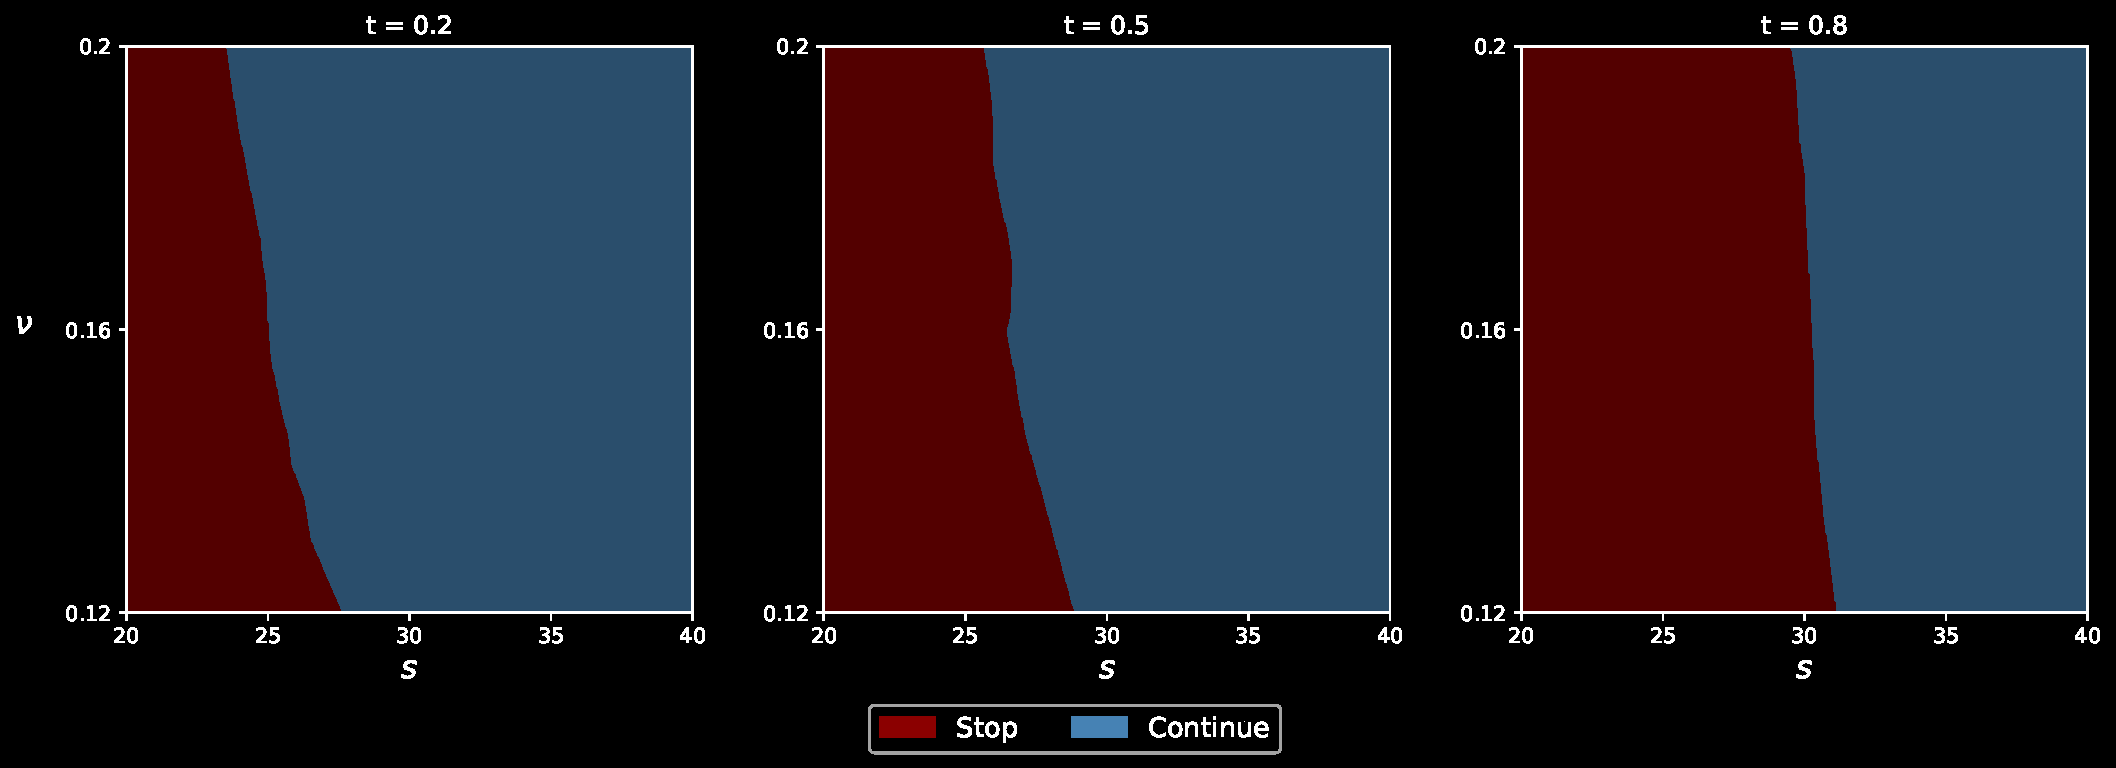
\includegraphics[scale = 0.42]{Figures/2DPlotHestonWide.pdf}
    \label{fig:heston1}
\end{figure}


\begin{figure}[t]
    \centering
     \caption{Stock price, variance and threshold process (Bermudan put, Heston model).}
    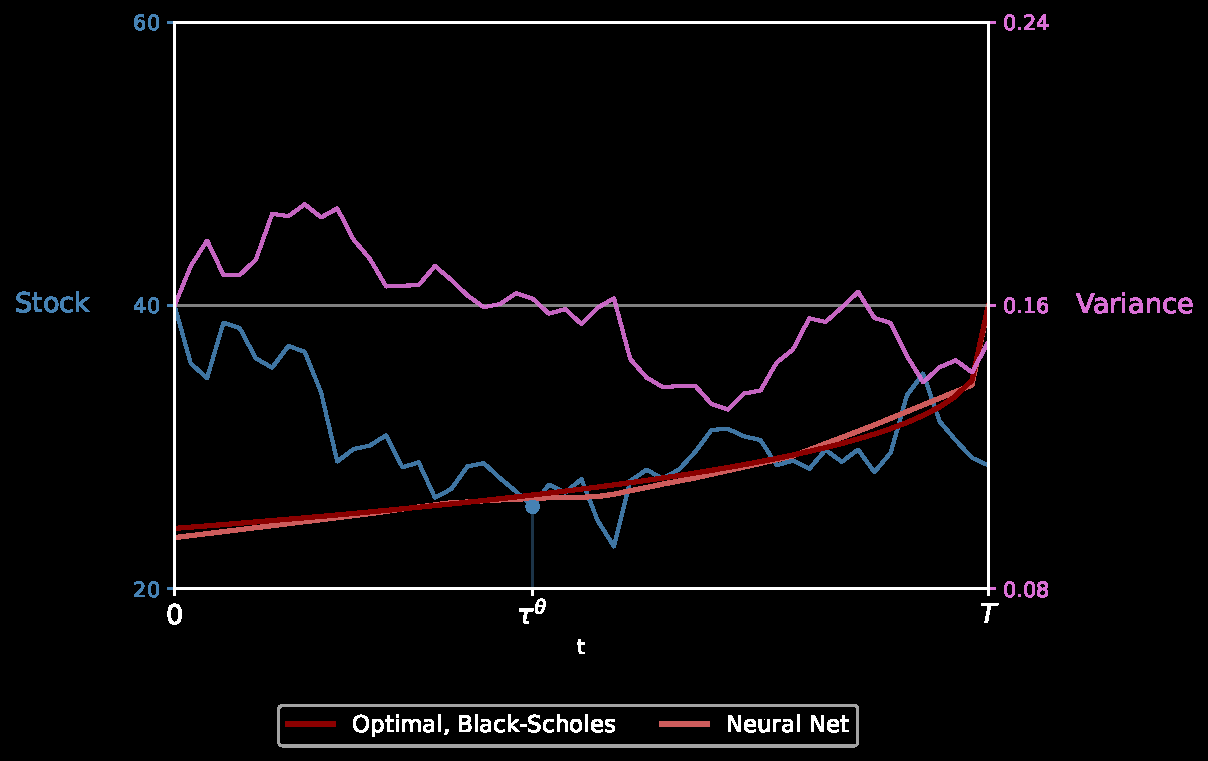
\includegraphics[scale = 0.42]{Figures/BdryHeston.pdf}
    \label{fig:heston2}
\end{figure}


\subsection{High-dimensional Max Option on Symmetric Assets}\label{sec:maxCallSym}
Let $\alpha(s) = \max_{i=1,...,d}s_i$, $\beta\equiv 0$, $\eta=1$ and consider the multi-dimensional Black-Scholes model with independent and symmetric assets, i.e. 
\begin{align}\label{eq:BSAsym}
    d S_t = \text{diag}(S_t) \left[ (r\mathds{1} - \delta)dt + \sigma dW_t\right],
\end{align}
where $W$ is Brownian motion in $\R^d$, $r \in \R ,\sigma > 0$ and $\delta \in \R_+^d$. We employ the parameters from Section of \cite{Becker2}, which are $s_0 =100 $, $r=5\%$, $\delta =10\%$ and $\sigma = 20 \%$. 

As both the payoff and assets are symmetric, it is easily shown that  $\calS_t$ is symmetric as well; see \cref{sec:symmetry}. This property can be exploited to reduce the dimension of our problem. Indeed, observe that it suffices to characterize the $t-$sections of the stopping region in the \textit{cone of ordered stocks}  
 $\calO = \{s\in \R_+^d \,|\, s_1 \geq \ldots \geq s_d\}$. We can therefore arrange $\Xi(S_t) = \frac{S_t}{\alpha(S_t)}\in [0,1]^d$ in decreasing order and give the outcome to $G(t,\cdot; \theta)$. If $\bar{S}_t \in \calO$ denotes the ordered version of $S_t$, then the last component of $\bar{S}_t$ are of little relevance to our stopping decision. 
 Indeed, over a short horizon, the maximum is  likely to be attained by the current best performing assets. %a stock having a high value today. 
 We can therefore set a cutoff $2 \le d' \ll d$ and feed the neural network with $(\frac{\bar{S}_{t,2}}{\alpha(S_t)},\ldots,\frac{\bar{S}_{t,d'}}{\alpha(S_t)})$ only.\footnote{Note that $\frac{\bar{S}_{t,1}}{\alpha(S_t)} \equiv 1$ is also removed from the neural network input as it doesn't carry any information.} Although one still needs to simulate $d$ assets, the size of the neural network can be significantly reduced, which in turn accelerates the training phase.  
 
 We illustrate this argument with $d=20$ assets and a cutoff of $d'=5$. 

\subsection{Max Option on $d=2$ Asymmetric Assets}\label{sec:maxCallAsym}
Consider the multi-dimensional Black-Scholes model, i.e. 
\begin{align}\label{eq:BSAsym}
    d S_t = \text{diag}(S_t) \left[ (r\mathds{1} - \delta)dt + \sigma dW_t\right],
\end{align}
where $W$ is Brownian motion in $\R^d$, $r \in \R ,\sigma > 0$ and $\delta \in \R_+^d$. 
Define the connected components $\calS^{(i)}_t = \calS_t \cap \{\alpha(s) = s_i\}$, $i=1,2$ and the involution   $\varsigma(s_1,s_2) := (s_2,s_1)$.  

\begin{proposition} Consider a max option on $d=2$ assets with $S$ having dynamics as in $\eqref{eq:BSAsym}$. IF $\delta_1 \ge \delta_2$, then $\varsigma(\calS^{(1)}_t) \subseteq \calS^{(2)}_t$. \rr{(to be verified numerically...)}
\end{proposition}

\begin{proof} (\bb{attempts...})
Let $t\in [0,T)$ and take any $\tau \in \calT_t$. Then, defining the event $B = \{S^{t,s_1}_{\tau,1} \ge  S^{t,s_2}_{\tau,2}\}$, this gives
\begin{align*}
    \E^{\Q}[D_{t,\tau} \varphi(S^{t,s}_{\tau}) ] &= \E^{\Q}[D_{t,\tau} (S^{t,s_1}_{\tau,1}-K)^+ \ \mathds{1}_{B} ] + \E^{\Q}[D_{t,\tau} (S^{t,s_2}_{\tau,2}-K)^+ \ \mathds{1}_{B^c} ]. 
\end{align*}
Since $\gamma := e^{(\delta_1-\delta_2)(\tau-t)} \le 1$, then  $\{\gamma S^{t,s_1}_{\tau,1} \ge  \gamma^{-1} S^{t,s_2}_{\tau,2}\} \subseteq B$. Moreover, note that $(\gamma S^{t,s_1}_{\tau,1},\gamma^{-1} S^{t,s_2}_{\tau,2}) \overset{d}{=} \varsigma(S^{t,\varsigma(s)}_{\tau})$. 
\begin{equation*}
    \E^{\Q}[D_{t,\tau} (S^{t,s_1}_{\tau,1}-K)^+ \ \mathds{1}_{B} ] \ge  \E^{\Q}\left[D_{t,\tau} (\gamma S^{t,s_1}_{\tau,1}-K)^+ \ \mathds{1}_{\{\gamma S^{t,s_1}_{\tau,1} \ge  \gamma^{-1} S^{t,s_2}_{\tau,2}\}} \right ] = \E^{\Q}[D_{t,\tau} ( S^{t,s_1}_{\tau,2}-K)^+ \ \mathds{1}_{B'} ],
\end{equation*}
with $B':= \{ S^{t,s_1}_{\tau,2} \ge  S^{t,s_2}_{\tau,1}\}$. On the other hand, note that $S^{t,s_2}_{\tau,2} \ge S^{t,s_1}_{\tau,1} \ge S^{t,s_2}_{\tau,1} $ on $B^c$. Hence, 
\begin{align*}
    \E^{\Q}[D_{t,\tau} (S^{t,s_2}_{\tau,2}-K)^+ \ \mathds{1}_{B^c} ] &\ge  \E^{\Q}[D_{t,\tau} (S^{t,s_2}_{\tau,1}-K)^+ \ \mathds{1}_{B^c} ]\\
    &\rr{\ge} \E^{\Q}[D_{t,\tau} (S^{t,s_2}_{\tau,1}-K)^+ \ \mathds{1}_{(B')^c} ].
\end{align*}
But $B^c \subseteq B$!

We would conclude: 
\begin{align*}
    \E^{\Q}[D_{t,\tau} \varphi(S^{t,s}_{\tau}) ] &\ge \E^{\Q}[D_{t,\tau} ( S^{t,s_1}_{\tau,2}-K)^+ \ \mathds{1}_{B'} ] + \E^{\Q}[D_{t,\tau} (S^{t,s_2}_{\tau,1}-K)^+ \ \mathds{1}_{(B')^c} ]\\ 
    &= \E^{\Q}[D_{t,\tau} \varphi(S^{t,\varsigma(s)}_{\tau}) ]. 
\end{align*}

...

To show: 
$$\E^{\Q}[ \varphi(S^{t,s}_{u}) ] \ge \E^{\Q}[ \varphi(S^{t,\varsigma(s)}_{u}) ], \quad \forall \ u \in [t,T].  $$
And multiply by $D_{t,u}$. 

E.g., use stochastic dominance $\alpha(S^{t,s}_{u}) \succ \alpha(S^{t,\varsigma(s)}_{u})$. And therefore, if $\varphi = \psi \circ \alpha$ with $\psi(a) \to 0$ as $a\to \infty$
\begin{align*}
    \E^{\Q}[\varphi(S^{t,s}_{u}) ] &= \int_0^{\infty} \psi(a) d\Q(\alpha(S^{t,s}_{u}) \le a) \\ 
    &=  - \int_0^{\infty} \Q(\alpha(S^{t,s}_{u}) \le a) d \psi(a) \\ 
    &\ge  - \int_0^{\infty} \Q(\alpha(S^{t,\varsigma(s)}_{u}) \le a) d \psi(a) \\ 
     &\ge  \E^{\Q}[\varphi(S^{t,\varsigma(s)}_{u}) ].
\end{align*}
 If needed,  use $\psi^N \uparrow \psi$  and the monotone convergence theorem.  
%$M^{t,s}_{u} \succ M^{t,\varsigma(s)}_{u} $, where $M^{t,s}_{u} = \alpha(S^{t,s}_{u})$. 
\end{proof}

\begin{figure}
    \centering
    \caption{Stopping and continuation regions (max option, $d=2$ assets, $T=3$).}
    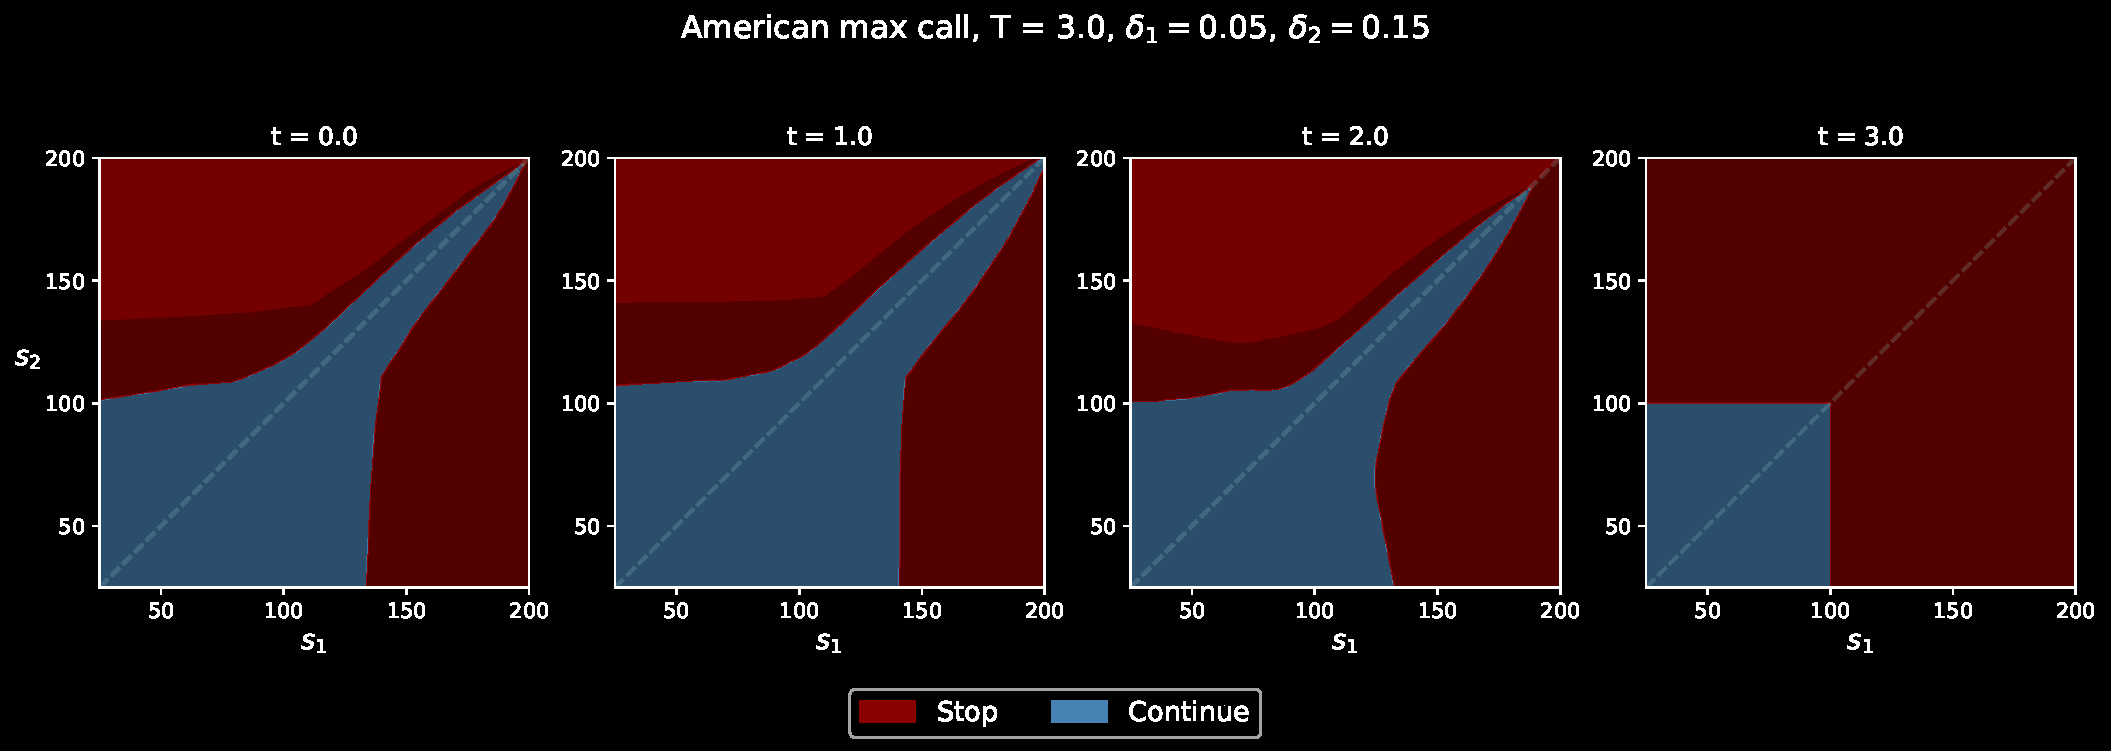
\includegraphics[scale = 0.42]{Figures/AsymMaxCall.pdf}
    \label{fig:asymCall}
    
    \scriptsize{
\textit{Notes: The light red region is the reflected image of $\calS_t^{(1)}$ through the diagonal, i.e. $\varsigma(\calS_t^{(1)})$.}} %This is to  illustrate that $\varsigma(\calS_t^{(1)}) \subseteq \calS_t^{(2)}$.  }}
\end{figure}

%\subsection{Spread Option}
%\subsection{Floating Strike Asian Option} \label{sec:Asian}
\subsection{Fixed Strike  Lookback Option} \label{sec:Lkbk}


